\documentclass[11pt]{article}
\usepackage[margin=1in]{geometry}
\usepackage{amsmath,amssymb,amsthm,mathtools}
\usepackage{booktabs,graphicx,hyperref,xcolor}
\usepackage[numbers,sort&compress]{natbib}

\newtheorem{theorem}{Theorem}
\newtheorem{proposition}{Proposition}
\theoremstyle{definition}
\newtheorem{definition}{Definition}
\newtheorem{remark}{Remark}

\newcommand{\R}{\mathbb{R}}
\newcommand{\X}{\mathcal{X}}
\newcommand{\Hk}{\mathcal{H}}
\newcommand{\inner}[2]{\langle #1, #2 \rangle}
\newcommand{\norm}[1]{\lVert #1 \rVert}
\newcommand{\E}{\mathbb{E}}
\DeclareMathOperator{\tr}{tr}
\DeclareMathOperator{\softmax}{softmax}

\title{\textbf{Multi-Scale Spectral Kernel Machines for Tabular Data}\thanks{Code available at
\url{https://github.com/asudjianto-xml/Spectral-Kernel}.}}
\author{Agus Sudjianto \and Aijun Zhang}
\date{\today}

\begin{document}
\maketitle

\begin{abstract}
We treat supervised learning as the construction of a kernel: once a positive-semidefinite
kernel is fixed, kernel ridge regression determines the estimator, so learning is the choice
of a data-adapted kernel. We develop the Multi-Scale Spectral Kernel Machine (MS-SKM), a
structured, inspectable kernel for tabular data, and study it as a ladder in which each rung
lifts one modeling restriction: from an additive model on fixed random Fourier features, to
learned frequencies, to a radial kernel on a per-coordinate spectral embedding, to feature
mixing, to multi-resolution banks fused on the simplex. Three results organize the design.
Interactions come from the kernel nonlinearity, not the linear mixer, which only rotates them
from axis-aligned to oblique. The convex multi-bank fuse is positive-semidefinite and
decomposes into one component per bank, whereas a linear mixer over banks collapses to a single
bank with the pooled frequencies---so the per-bank bandwidth is what fusion adds. A parameter
accounting makes the per-band frequency count the overfitting axis and the bank count the
multi-scale axis. The ladder isolates each effect on real data, and a variational head trains
the same kernel by a sparse Gaussian-process ELBO to return a calibrated predictive
distribution.
\end{abstract}

\vskip 0.1in
\noindent\textbf{Keywords:} kernel methods, spectral kernels, Gaussian processes, tabular data,
kernel ridge regression, additive models, multi-resolution learning, variational inference

\section{Introduction}
A prediction at a query point borrows strength from training points through a notion of
similarity, the \emph{kernel}. Kernel methods fix this object a priori, tree ensembles induce
it through a learned partition, and neural networks learn a representation whose inner product
is a kernel. Gradient-boosted decision trees remain the default for tabular data and frequently
outperform deep models \citep{chen2016xgboost,ke2017lightgbm,prokhorenkova2018catboost,grinsztajn2022}.
Taking the kernel itself as the primitive, we ask what a trainable kernel for tabular data
should look like, and we build it from the spectral domain as a competitive learned-kernel
alternative.

Learnable spectral kernels are not new: spectral-mixture kernels model a spectral density
\citep{wilson2013}, sparse-spectrum Gaussian processes learn finite spectral atoms
\citep{lazarogredilla2010} and \`a-la-carte kernels learn groups of fast frequencies
\citep{yang2015}. Our contribution is an \emph{arrangement} of these decisions into a tabular
inductive bias and a \emph{ladder} that makes each decision's contribution measurable. Each
rung lifts one restriction:
\begin{enumerate}\itemsep1pt
\item \textbf{Rung 0 --- fixed-frequency additive model.} Per-coordinate random Fourier
features with a linear readout. The frequencies are fixed, the model is additive, there is no
kernel. This is a generalized additive model \citep{hastie1990} solved in closed form.
\item \textbf{Rung A --- learned frequencies, still additive.} The frequencies are learned. The
model stays additive and kernel-free.
\item \textbf{Rung B --- the kernel, no mixing.} A radial base kernel on a per-feature spectral
embedding, with a block-diagonal encoder so no feature is mixed into another.
\item \textbf{Rung 1 --- full mixing.} The encoder mixes features. The kernel now sees oblique
interactions.
\item \textbf{Rung 2 --- multi-resolution banks.} Frequencies are partitioned into $H$ banks,
each with its own bandwidth, convex-fused on the simplex.
\end{enumerate}
The ladder is the methodological point. A single accuracy number hides whether a model needs
interactions at all, whether they are axis-aligned or oblique and whether it needs multiple
scales or only more frequencies. Lifting one restriction at a time answers each question
separately, on the same data and the same training machinery.

\paragraph{Contributions.} We are explicit about what is \emph{proven}, what is a
\emph{diagnostic}, and what is a \emph{conjecture supported by a sweep}.
\begin{enumerate}\itemsep2pt
\item \emph{(Proven.)} The per-coordinate feature map realizes a sum of one-dimensional
spectral-mixture kernels (Prop.~\ref{prop:additive}), dense in the additive-stationary class
between additive Gaussian processes \citep{duvenaud2011} and spectral-mixture kernels
\citep{wilson2013}.
\item \emph{(Proven / diagnostic.)} Interactions come from the radial base kernel, not the
mixer (Prop.~\ref{prop:interaction}). A linear mixer is a learned metric $W^\top W$ whose
off-diagonal blocks are an inspectable diagnostic of \emph{metric} interaction; with the mixer
block-diagonal the kernel is still non-additive.
\item \emph{(Proven.)} The convex multi-bank fuse is positive-semidefinite and decomposes
exactly into one component per bank in the sum RKHS (Prop.~\ref{prop:fusion}), and a single
linear mixer over banks collapses to one bank with the pooled frequencies
(Prop.~\ref{prop:collapse})---so the per-bank bandwidth, not the bank count, is what convex
fusion adds.
\item \emph{(Accounting + sweep.)} The dominant parameter count scales with the per-band
frequency count $K$ and is independent of the bank count $H$ (Prop.~\ref{prop:capacity}); we
observe $K$ to be the overfitting axis and $H$ the multi-scale axis.
\item \emph{(Whittle / diagnostic.)} A one-dimensional criterion for when learning the
frequencies helps (Prop.~\ref{prop:freqlearn}): the gradient on a frequency atom is
proportional to the local residual spectral mass, vanishing on flat spectra and active on
peaked ones.
\item \emph{(Predictive distribution.)} A variational head (Sec.~\ref{sec:elbo}) that trains the
same learned kernel by the ELBO of a sparse Gaussian process \citep{titsias2009,hensman2013},
giving a calibrated Gaussian predictive distribution rather than a point.
\item \emph{(Interpretability.)} Because the kernel is learned, its parameters are the
explanation: automatic relevance determination (ARD) gives a per-feature importance and the encoder metric $W^\top W$ gives
pairwise metric interactions, read directly off the fitted model with no surrogate
(Sec.~\ref{sec:exp}).
\item An open-source implementation and an ablation ladder that isolates each effect on real
tabular data.
\end{enumerate}

\section{The kernel is the object of learning}\label{sec:setup}
Let $\{(x_i,y_i)\}_{i=1}^n$ with $x_i\in\X\subseteq\R^d$. A symmetric positive-semidefinite
(PSD) kernel $k$ induces a reproducing-kernel Hilbert space (RKHS) $\Hk_k$ and a Gaussian-process
prior $f\sim\mathcal{GP}(0,k)$. Regularized risk minimization in $\Hk_k$ has, by the representer
theorem, the finite solution $\hat f(\cdot)=\sum_i\alpha_i k(\cdot,x_i)$; for squared loss this
is kernel ridge regression (KRR), which coincides with the GP posterior mean
\begin{equation}
\hat f(x)=k(x,X)\,(K+\lambda I)^{-1}y,\qquad K_{ij}=k(x_i,x_j).
\label{eq:krr}
\end{equation}
The estimator \eqref{eq:krr} is a fixed functional of $k$; the learning problem is the choice
of $k$ from a parameterized family $\{k_\theta\}$, here by empirical Bayes over $\theta$
\citep{rw2006}. We therefore study the admissible $k_\theta$ directly.

\section{A per-coordinate spectral construction}\label{sec:spectral}
A continuous stationary kernel $k(x,x')=\kappa(x-x')$ is PSD if and only if $\kappa$ is the
Fourier transform of a finite nonnegative measure $\mu$, the spectral measure (Bochner). Kernel
learning restricted to the stationary class is spectral-measure estimation \citep{wilson2013}.
Rather than estimate $\mu$ on $\R^d$ jointly, MS-SKM estimates a measure on each coordinate.
Fix per-coordinate frequencies $\{\omega_{j,k}\}_{k=1}^K$, nonnegative amplitudes $\{a_{j,k}\}$
and a per-coordinate automatic-relevance-determination (ARD) scale $s_j>0$
\citep{neal1996,mackay1996,rw2006}, and define the feature map with components
\begin{equation}
\psi(x)_{j,k}=a_{j,k}\big[\cos(2\pi s_j\,\omega_{j,k}\,x_j),\ \sin(2\pi s_j\,\omega_{j,k}\,x_j)\big],
\qquad j=1,\dots,d,\ k=1,\dots,K.
\label{eq:psi}
\end{equation}
Unlike random Fourier features \citep{rahimi2007}, where each feature is $\cos(\omega^\top x)$
with $\omega\in\R^d$ mixing all coordinates, \eqref{eq:psi} is a one-dimensional Fourier
expansion applied independently to each coordinate---the periodic numerical embedding of
tabular deep learning \citep{gorishniy2022,ye2024}, read spectrally.

\begin{proposition}[Additive spectral-mixture realization]\label{prop:additive}
The inner product of \eqref{eq:psi} is the additive kernel
\begin{equation}
\inner{\psi(x)}{\psi(x')}=\sum_{j=1}^d\sum_{k=1}^K a_{j,k}^2\,
\cos\!\big(2\pi s_j\omega_{j,k}(x_j-x_j')\big)=\sum_{j=1}^d\kappa_j(x_j-x_j'),
\label{eq:additive}
\end{equation}
where each $\kappa_j$ is a one-dimensional stationary kernel with atomic spectral measure
\begin{equation*}
\mu_j=\tfrac12\sum_k a_{j,k}^2\big(\delta_{s_j\omega_{j,k}}+\delta_{-s_j\omega_{j,k}}\big).
\end{equation*}
Hence $\psi$ realizes a sum of per-coordinate spectral-mixture kernels and is PSD. As $K\to\infty$ with
$\{a_{j,k}^2\}$ a consistent quadrature of a density $p_j$, each $\kappa_j$ converges to the
kernel of $p_j$, so the family is dense in the additive-stationary class
\citep{wilson2013,duvenaud2011}.
\end{proposition}
\begin{proof}
The identity $\cos A\cos B+\sin A\sin B=\cos(A-B)$ with $A=2\pi s_j\omega_{j,k}x_j$ and
$B=2\pi s_j\omega_{j,k}x_j'$ gives the cosine term after the $a_{j,k}^2$ weighting; summing
over $k$ then $j$ yields \eqref{eq:additive}. Each $\mu_j$ is finite, nonnegative and symmetric,
so by Bochner $\kappa_j$ is PSD; a sum of PSD kernels in disjoint coordinates is PSD. Density is
coordinatewise \citep{wilson2013} and additive \citep{duvenaud2011}.
\end{proof}

With a linear readout $f(x)=\beta^\top\psi(x)$ this is rung~0 (frequencies fixed, solved in
closed form) and rung~A (frequencies learned by gradient descent). In both, the readout weights
are the per-frequency amplitudes, the model is additive, and there is no kernel.

\section{Interactions from the kernel, not the mixer}\label{sec:warp}
The additive map \eqref{eq:additive} has no cross-coordinate interactions. We introduce a single
linear encoder $W$, $\phi(x)=W\psi(x)$, and a Laplace base kernel,
\begin{equation}
k_\theta(x,x')=\exp\!\big(-\norm{W(\psi(x)-\psi(x'))}_2/T\big),\qquad \theta=(s,\omega,a,W,T),
\label{eq:kernel}
\end{equation}
the deep-kernel construction \citep{wilson2016} with a shallow, linear warp on additive spectral
features. It is essential to separate three notions of interaction. \emph{Metric:}
cross-coordinate blocks of $M=W^\top W$. \emph{Kernel:} failure of $k_\theta$ to be additive.
\emph{Functional:} a non-additive contribution to the fitted predictor.

\begin{proposition}[Where interactions come from]\label{prop:interaction}
Let $\Delta\psi=\psi(x)-\psi(x')$, blocked by coordinate. Then $k_\theta$ in \eqref{eq:kernel}
is PSD and
\begin{equation}
\norm{W\Delta\psi}_2^2=\Delta\psi^\top M\Delta\psi
=\sum_j\Delta\psi^{(j)\top}M_{jj}\Delta\psi^{(j)}
+\sum_{j\neq j'}\Delta\psi^{(j)\top}M_{jj'}\Delta\psi^{(j')},\quad M=W^\top W\succeq0.
\end{equation}
Consequently \textup{(i)} a linear readout on $\psi$ (no kernel) is additive for any $W$, since
$\beta^\top W\psi$ is linear in $\psi$ and each block of $\psi$ depends on one coordinate, so a
linear mixer neither creates nor removes interactions; \textup{(ii)} with $M$ block-diagonal the
kernel is still non-additive, because $\exp(-\sqrt{\sum_j d_j^2}/T)$ does not factor over the
$d_j$, so kernel and functional interactions are present with zero metric interaction; \textup{(iii)}
the off-diagonal blocks $M_{jj'}$ are an inspectable diagnostic of \emph{metric} interaction, and
mixing rotates the interactions the kernel forms from axis-aligned to oblique.
\end{proposition}
\begin{proof}
$\exp(-\norm{Lz}/T)$ is PSD for any matrix $L$ and $T>0$: $\exp(-\norm{u}/T)$ is PSD
(Mat\'ern-$\tfrac12$) and composition with a linear map preserves positive-definiteness; take
$L=W$. The decomposition is the block expansion of $\Delta\psi^\top W^\top W\Delta\psi$. Claim
(i) is immediate from linearity. For (ii), with $M$ block-diagonal the squared distance is
$\sum_j d_j^2$ but the Laplace map of its square root does not separate.
\end{proof}

\begin{proposition}[Universality]\label{prop:universal}
If the per-coordinate bank separates points and $\phi=W\psi$ is injective on the compact domain,
then $k_\theta$ is universal: its RKHS is dense in $C(\X)$ \citep{micchelli2006}. Every
continuous function, and thus every interaction, is approximable; the additive base is not a
structural barrier. Interactions enter through the radial nonlinearity acting on linear
projections of the univariate features, exactly as an RBF kernel on raw inputs realizes
interactions despite a coordinatewise input.
\end{proposition}

Rung~B is \eqref{eq:kernel} with $W$ block-diagonal (a per-feature encoder, no mixing); rung~1
is \eqref{eq:kernel} with $W$ full. By Prop.~\ref{prop:interaction} rung~B already has
interactions, axis-aligned; rung~1 makes them oblique.

\section{Multi-resolution fusion}\label{sec:fusion}
We replicate the construction in $H$ banks. Bank $h$ carries its own frequencies $\omega_h$ and
amplitudes $a_h$ initialized on a band of a log-spaced partition of the frequency range, its own
bandwidth $T_h$, and a shared encoder $W$ applied to each bank's own $2dK$-dimensional feature
vector $\psi_h(x)$ separately. The banks are fused convexly,
\begin{equation}
k(x,x')=\sum_{h=1}^H w_h\,k_h(x,x'),\qquad w=\softmax(\cdot)\in\Delta^{H-1},
\label{eq:fuse}
\end{equation}
with $k_h$ as in \eqref{eq:kernel} using $(\omega_h,a_h,T_h)$. This is rung~2.

\begin{proposition}[Closure and decomposition]\label{prop:fusion}
For $w_h\ge0$, $k$ in \eqref{eq:fuse} is PSD. The fused KRR fit decomposes exactly into one
component per bank,
\begin{equation}
\hat g_h=w_h K_h(K+\lambda I)^{-1}y,\qquad \textstyle\sum_h\hat g_h=\hat f,
\label{eq:components}
\end{equation}
and, by Aronszajn's sum-of-kernels theorem \citep{aronszajn1950,berlinet2004}, the RKHS of
$k=\sum_h w_h k_h$ is the sum space $\sum_h\Hk_{k_h}$ with the infimal-convolution norm
$\norm{f}_{\Hk_k}^2=\min_{f=\sum_h g_h}\sum_h\frac1{w_h}\norm{g_h}_{\Hk_{k_h}}^2$. If each bank
is normalized ($k_h(x,x)=1$) the posterior mean is invariant along $(w,\lambda)\mapsto(\alpha
w,\alpha\lambda)$, so the simplex fixes the mixture scale.
\end{proposition}
\begin{proof}
A nonnegative combination of PSD matrices is PSD. Equation \eqref{eq:components} is Gaussian
conditioning: with independent priors $g_h\sim\mathcal{GP}(0,w_h k_h)$ and $\mathrm{Cov}(g_h,y)=w_h
K_h$, $\E[g_h\mid y]=w_h K_h(K+\lambda I)^{-1}y$, and $\sum_h w_h K_h=K$. The sum-RKHS norm is
Aronszajn's theorem. Invariance follows from $\alpha K(\alpha K+\alpha\lambda I)^{-1}=K(K+\lambda
I)^{-1}$.
\end{proof}

The decomposition is the rigorous statement that a convex fuse of banks at different scales is
\emph{not} reducible to a single kernel. The next proposition shows what the alternative ---
mixing the banks linearly --- actually is.

\begin{proposition}[A linear mixer over banks collapses to one bank]\label{prop:collapse}
Let the banks be combined by a single linear map applied to the concatenation
$[\psi_1(x);\dots;\psi_H(x)]$, followed by one base kernel of bandwidth $T$. The concatenation of
$H$ banks of $K$ frequencies is a single bank of $HK$ frequencies, and one linear encoder over it
is the encoder of \eqref{eq:kernel} with $K'=HK$. Hence ``$H$ banks $+$ one linear mixer'' equals
``one bank with $K'=HK$ frequencies'': a single kernel with a single bandwidth. The per-bank
bandwidths $T_h$ of \eqref{eq:fuse} are absent from this construction, and a single bandwidth
cannot span frequencies of widely separated scale.
\end{proposition}

\begin{proposition}[Parameter accounting]\label{prop:capacity}
With $H$ banks of $K$ frequencies each and the shared per-bank encoder $W\in\R^{d_\phi\times2dK}$,
the free-parameter count is
\begin{equation}
\underbrace{H\cdot d\cdot 2K}_{\text{bank spectra}}\ +\ \underbrace{d\cdot 2K\cdot d_\phi}_{\text{shared encoder }W}\ +\ O(H),
\label{eq:paramcount}
\end{equation}
so the dominant encoder term scales with $K$ and is independent of $H$.
\end{proposition}

\begin{remark}[Banks versus frequencies]\label{rem:capacity}
The two axes generalize differently. Increasing $H$ adds multi-resolution structure on a shared
basis, gated by the simplex weights $w_h$. Increasing $K$ widens the dominant ungated encoder
\eqref{eq:paramcount} and packs more frequencies into a band whose amplitude envelope is already a
smooth quadrature (Prop.~\ref{prop:additive}). We therefore expect $K$ to be the overfitting axis
and $H$ the multi-scale axis, a multi-resolution echo of the frequency-overfitting of
\citep{galturner2015}. The selection of $w$ here is by marginal likelihood, jointly with the
banks; selecting $w$ by an unbiased risk estimate over fixed banks
\citep{stein1981,golub1979gcv} would inherit the oracle guarantee that convex fusion is never
worse than the best single bank, and is a natural alternative.
\end{remark}

\section{When does learning the frequencies help?}\label{sec:freqlearn}
Sparse-spectrum methods learn $\omega$ by marginal likelihood and overfit on smooth targets
\citep{galturner2015,lazarogredilla2010}. We give a partial criterion in the cleanest setting,
one-dimensional regression, and use it as a tabular diagnostic.

\begin{proposition}[Frequency-learning gradient, 1-D Whittle regime]\label{prop:freqlearn}
Under the Whittle approximation to the Gaussian log-likelihood, with model spectrum
$S_\theta(\omega)=\lambda+\sum_k a_k^2 g(\omega-\omega_k)$, the gradient moving an atom is
\begin{equation}
\frac{\partial\mathcal{L}}{\partial\omega_k}\ \propto\ a_k^2\,\partial_\omega r(\omega)\big|_{\omega_k},
\qquad r(\omega)=\hat p(\omega)-\textstyle\sum_{k'}a_{k'}^2g(\omega-\omega_{k'}),
\end{equation}
the residual spectral density ($\hat p$ the periodogram, $g$ a fixed atom kernel). If $\hat p$ is
locally flat the atoms do not move and a fixed grid is already a consistent quadrature; if $\hat p$
is peaked the atoms migrate to the lines and a learned grid strictly improves the fit.
\end{proposition}
\begin{proof}[Sketch]
Differentiate $-\tfrac12\int[\log S_\theta+\hat p/S_\theta]d\omega$ in $\omega_k$ using
$\partial S_\theta/\partial\omega_k=-a_k^2 g'(\omega-\omega_k)$; the leading term is
$a_k^2\partial_\omega r(\omega_k)$.
\end{proof}

For multivariate tabular data the per-coordinate spectral density is not canonically defined, so
we read this as a diagnostic: learning the frequencies helps in proportion to per-coordinate
spectral peakedness. This is consistent with the smooth-versus-periodic reversal in
Section~\ref{sec:exp}.

\section{Training and inference}\label{sec:decode}
Hyperparameters $\theta$ are fit by the negative log marginal likelihood
$\mathcal{L}=\tfrac12 y^\top(K+\lambda I)^{-1}y+\tfrac12\log\lvert K+\lambda I\rvert+\text{const}$,
optimized by gradient descent on random support subsets (Cholesky in double precision, autograd);
the noise $\lambda$ is the learned ridge. Prediction is full-train KRR \eqref{eq:krr}, solved by a
truncated Lanczos tridiagonalization \citep{lanczos1950} so the cost is a handful of matrix-vector
products rather than a dense factorization. The frequencies and amplitudes are learned, never
frozen, so the construction is not random Fourier features: we learn the kernel rather than
approximate a fixed one. The feature and label scalers are fit on train, the ridge and the
calibration temperature on a validation fold, and test data is touched only at prediction.

\section{Predictive distributions via a variational bound}\label{sec:elbo}
The NLML objective with the KRR decode returns the Gaussian-process posterior mean --- a point
prediction. The exact GP posterior also has a closed-form predictive variance, but it requires a
dense solve and is tied to the Gaussian likelihood. To obtain a predictive distribution that
scales by minibatching and extends to non-Gaussian likelihoods, we train the same learned kernel
by the evidence lower bound (ELBO) of a sparse variational Gaussian process
\citep{titsias2009,hensman2013}.

Place $M$ inducing inputs $Z$ with prior $p(u)=\mathcal N(0,K_{ZZ})$, and a whitened variational
posterior $q(u)=\mathcal N(L m,\,L S L^\top)$ with $L=\mathrm{chol}(K_{ZZ})$. The variational
marginal at a point is $q(f_i)=\mathcal N(\mu_i,s_i^2)$ with
\begin{equation}
\mu_i=b_i^\top m,\qquad s_i^2=k_{ii}-b_i^\top(I-S)\,b_i,\qquad b_i=L^{-1}k(Z,x_i),
\end{equation}
and the kernel's unit diagonal gives $k_{ii}=1$. For a Gaussian likelihood with noise $\sigma^2$
the bound is
\begin{equation}
\mathrm{ELBO}=\sum_{i}\Big[\log\mathcal N(y_i\mid\mu_i,\sigma^2)-\tfrac{s_i^2}{2\sigma^2}\Big]
-\mathrm{KL}\big(q(u)\,\|\,p(u)\big),\quad
\mathrm{KL}=\tfrac12\big[\tr S+\norm{m}^2-M-\log\lvert S\rvert\big].
\end{equation}
The spectral parameters, the inducing inputs $Z$ and the variational parameters $(m,S,\sigma^2)$
are learned jointly by maximizing the ELBO on minibatches. The predictive distribution at $x^\star$
is Gaussian, $\mathcal N(\mu^\star,\,s^{\star2}+\sigma^2)$, so every prediction carries a variance.

The intervals are calibrated. On California Housing the $90\%$ and $95\%$ central predictive
intervals cover $0.93$ and $0.95$ of held-out points; on a one-dimensional series with a held-out
gap the predictive standard deviation grows from in-sample through the gap to extrapolation, the
expected Gaussian-process behavior. The sparse $M$-point head reaches $R^2\approx0.84$ where the
exact decode reaches $0.88$. The same bound extends to a Bernoulli or softmax likelihood for
classification.

\section{Experiments}\label{sec:exp}
We use California Housing (regression, $n{=}20{,}640$, $d{=}8$) and Breast Cancer (binary,
$n{=}569$, $d{=}30$) from scikit-learn, and an hourly bike-sharing series (regression, periodic),
each with a held-out $20\%$ test split; the remaining data is split into train and validation for
early stopping and the ridge. Classification uses one-hot KRR with a temperature-scaled
posterior. The kernel is Laplace, $K=16$ frequencies per feature per bank unless swept,
$d_\phi=128$.

\paragraph{An illustrative 2-D example.} Figure~\ref{fig:moons} fits the ladder and a tuned
CatBoost on \texttt{make\_moons}, two interleaving crescents whose separation needs an oblique
interaction. The additive rungs (0, A) draw blocky, near-separable boundaries; the boundary
curves the moment the kernel appears (rung B), feature mixing (rung 1) wraps it obliquely around
both crescents and CatBoost draws an axis-aligned staircase. Accuracy sits at the noise floor, so
the metrics (Table~\ref{tab:moons}) read through the boundary: AUC saturates, the kernel rungs win
on F1 and Brier, and CatBoost --- comparable on AUC --- has markedly worse Brier and log loss, the
signature of an accurate ranker with overconfident probabilities. The variational head
(Sec.~\ref{sec:elbo}) turns the same kernel into a predictive distribution
(Figure~\ref{fig:moons-unc}): the predictive standard deviation is low over the data-covered
crescents and rises in the empty regions, the epistemic uncertainty of a Gaussian process.

\begin{figure}[t]\centering
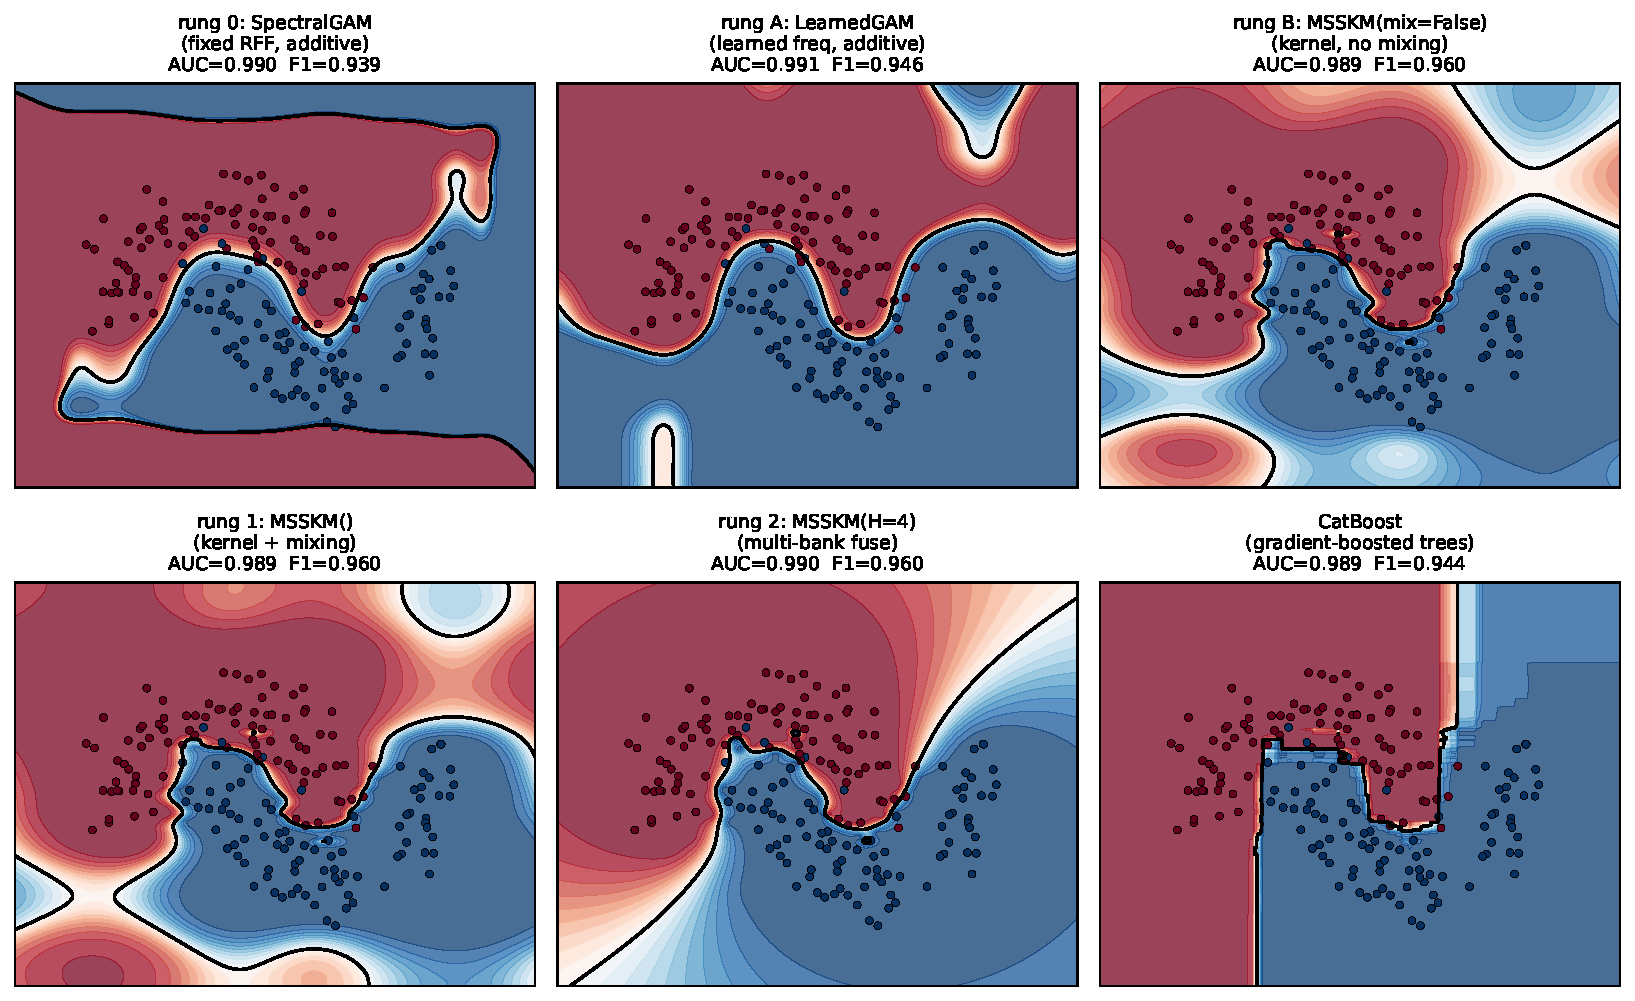
\includegraphics[width=\textwidth]{figures/moons_boundaries.pdf}
\caption{Decision boundaries on \texttt{make\_moons} (shading is $P(\text{class }1)$, black line the
$0.5$ boundary, dots the test set). Additive rungs give blocky separable boundaries; the kernel
curves them (rung B), mixing makes them oblique (rung 1); CatBoost is an axis-aligned staircase.}
\label{fig:moons}
\end{figure}

\begin{table}[t]\centering
\caption{\texttt{make\_moons} test metrics. AUC and F1 higher is better; Brier and log loss lower
is better. AUC saturates; the kernel rungs lead on F1 and Brier, and CatBoost is the least
calibrated (highest Brier and log loss) despite a comparable AUC.}
\label{tab:moons}
\begin{tabular}{lcccc}
\toprule
model & AUC & F1 & Brier & LogLoss \\
\midrule
rung 0: SpectralGAM        & 0.9895 & 0.9385 & 0.0430 & 0.1386 \\
rung A: LearnedGAM         & 0.9907 & 0.9457 & 0.0430 & 0.1537 \\
rung B: MSSKM(mix=False)   & 0.9888 & 0.9605 & 0.0358 & 0.1444 \\
rung 1: MSSKM()            & 0.9889 & 0.9605 & 0.0350 & 0.1393 \\
rung 2: MSSKM($H{=}4$)     & 0.9896 & 0.9605 & 0.0367 & 0.1423 \\
CatBoost                   & 0.9893 & 0.9444 & 0.0467 & 0.2011 \\
\bottomrule
\end{tabular}
\end{table}

\begin{figure}[t]\centering
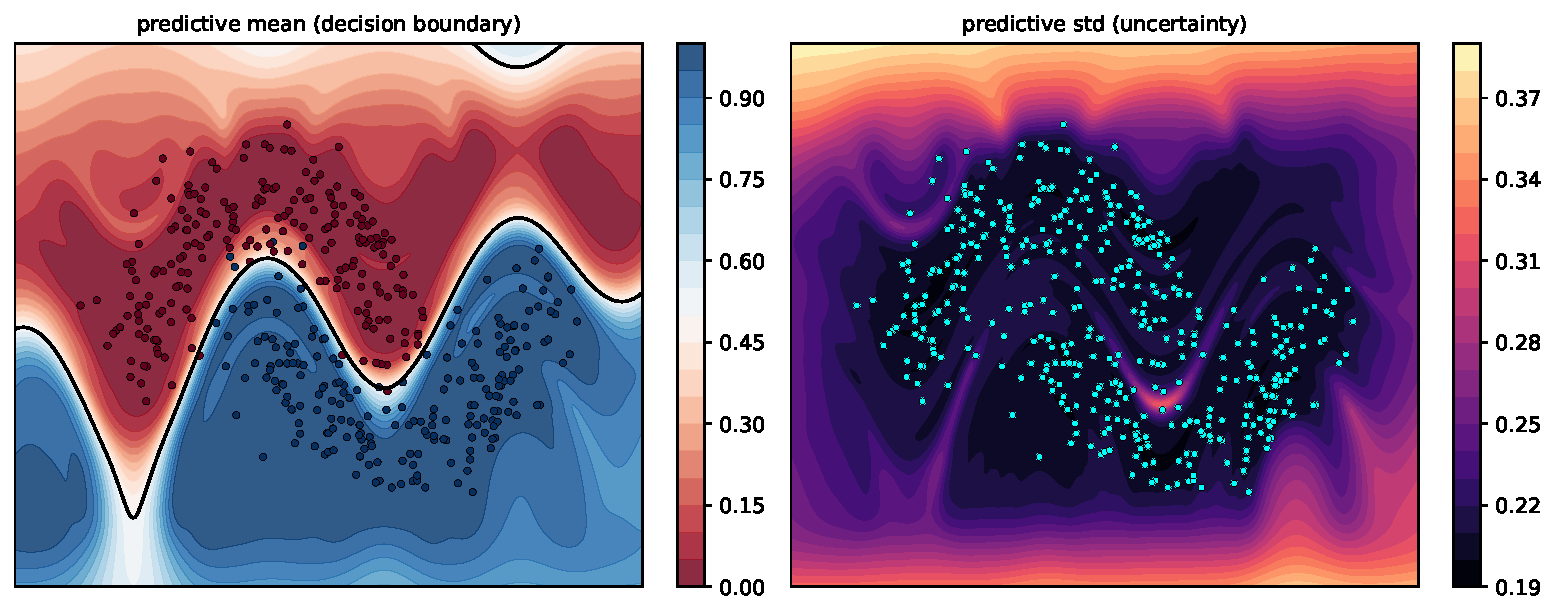
\includegraphics[width=0.86\textwidth]{figures/moons_uncertainty.pdf}
\caption{The variational (ELBO) head on \texttt{make\_moons}, regressing the $0/1$ labels. Left:
predictive mean with the $0.5$ boundary. Right: predictive standard deviation --- low over the
two crescents where there is data, high in the empty regions. This is the latent predictive
spread, not a calibrated Bernoulli posterior; a classification likelihood is future work.}
\label{fig:moons-unc}
\end{figure}

\paragraph{The ladder decomposition.} Table~\ref{tab:ladder} reports each rung. On California the
gain over the additive model is almost entirely the kernel and almost entirely axis-aligned:
rung~B (kernel, no mixing) recovers $0.711\to0.873$ of the $0.711\to0.876$ total, and the oblique
mixing of rung~1 adds $0.003$. On Breast Cancer the reverse holds: the kernel with no mixing adds
nothing ($0.947\to0.947$) and the whole gain is the oblique mixing ($\to0.965$). The interactions
California needs are axis-aligned and reached by the radial kernel without mixing
(Prop.~\ref{prop:interaction}); those Breast Cancer needs live along learned feature combinations.

\begin{table}[t]\centering
\caption{The ladder, test metric (R$^2$ for California, accuracy for Breast Cancer). Each rung
lifts one restriction.}
\label{tab:ladder}
\begin{tabular}{llcc}
\toprule
rung & model & California R$^2$ & Breast Cancer acc \\
\midrule
0 & fixed RFF, additive, no kernel        & 0.713 & 0.947 \\
A & learned freq, additive, no kernel     & 0.711 & 0.947 \\
B & kernel, no mixing (block-diagonal $W$)& 0.873 & 0.947 \\
1 & kernel, full mixing                   & 0.876 & 0.965 \\
2 & multi-bank convex fuse ($H{=}4$)      & 0.885 & 0.956 \\
\bottomrule
\end{tabular}
\end{table}

\paragraph{Learning the frequencies (rung 0 vs A).} On smooth California, learning the
frequencies moves test R$^2$ by $<0.01$ ($0.713\to0.711$), and on Breast Cancer it is unchanged.
This is the flat-spectrum case of Prop.~\ref{prop:freqlearn}: a fixed grid is already a consistent
quadrature and the amplitudes carry the information.

\paragraph{Convex fuse versus a linear mixer (Prop.~\ref{prop:collapse}).} At a matched frequency
budget of $256$ per feature, one bank with $K{=}256$ (a linear mixer over the pooled frequencies)
matches one bank with $K{=}64$ on California ($0.876$ vs $0.876$) and is worse on Breast Cancer
($0.939$ vs $0.965$, overfitting), while splitting the same $256$ frequencies into four
convex-fused banks of $K{=}64$ reaches $0.885$ on California. Pooling frequencies into one kernel
does nothing; the gain is the per-bank bandwidth of the convex fuse, exactly
Prop.~\ref{prop:collapse}.

\paragraph{The $H\times K$ sweep.} Table~\ref{tab:sweep} sweeps banks against per-band
frequencies, and bears out Prop.~\ref{prop:capacity} and Remark~\ref{rem:capacity}. Along each
row (fixed $H$, increasing $K$) the metric is flat or declines: extra frequencies in one bank do
not help and the ungated encoder eventually overfits, sharpest on small Breast Cancer where
$K{=}32$ at $H{=}8$ falls back. Down each column (fixed $K$, increasing $H$) the multi-scale
regressions improve monotonically (California $0.873\to0.885$, Bike-hourly $0.943\to0.954$ at
$K{=}8$), while small Breast Cancer is flat-to-worse, its near-uniform fusion weights signalling no
multi-scale structure to exploit. The best corner is moderate $K$ with larger $H$: capacity comes
from banks, not from frequencies per bank.

\begin{table}[t]\centering
\caption{Test metric over $H$ (banks) $\times$ $K$ (frequencies per feature): R$^2$ for California
and Bike-hourly, accuracy for Breast Cancer. \textbf{Bold} is the configuration selected on the
validation fold and evaluated once on test. Generated by \texttt{benchmarks/sweep\_hk.py}.}
\label{tab:sweep}
\begin{tabular}{llccc}
\toprule
Dataset & $H$ & $K{=}8$ & $K{=}16$ & $K{=}32$ \\
\midrule
California (R$^2$)   & 1 & 0.873          & 0.875          & 0.875 \\
                     & 2 & 0.881          & 0.880          & 0.882 \\
                     & 4 & \textbf{0.883} & 0.883          & 0.882 \\
                     & 8 & 0.885          & 0.884          & 0.884 \\
\midrule
Breast Cancer (acc)  & 1 & 0.956          & 0.974          & 0.956 \\
                     & 2 & 0.965          & 0.965          & \textbf{0.982} \\
                     & 4 & 0.956          & 0.956          & 0.965 \\
                     & 8 & 0.947          & 0.974          & 0.965 \\
\midrule
Bike-hourly (R$^2$)  & 1 & 0.943          & 0.942          & 0.944 \\
                     & 2 & 0.951          & 0.952          & 0.946 \\
                     & 4 & 0.953          & 0.953          & 0.953 \\
                     & 8 & 0.954          & \textbf{0.956} & 0.953 \\
\bottomrule
\end{tabular}
\end{table}

\paragraph{Interpretability from the learned kernel.} The kernel is learned, so its parameters
\emph{are} the explanation: the quantities below are closed-form functionals of the fitted
parameters, computed exactly, with no surrogate model, perturbation, sampling or permutation
(Figure~\ref{fig:interpret}). \emph{Relevance.} The scale $s_j$ in \eqref{eq:psi} is the inverse
length scale of feature $j$: it multiplies $x_j$ inside every $\cos/\sin(2\pi s_j\omega_{j,k}x_j)$,
so as $s_j\to0$ those coordinates flatten to constants and feature $j$ leaves the kernel. Training
therefore drives $s_j$ small for uninformative features and large for relevant ones, which is
automatic relevance determination \citep{neal1996,mackay1996}. \emph{Importance.} Relevance alone
ignores how much spectral energy a feature carries, so we score feature $j$ by how strongly the
embedding turns with it. Differentiating \eqref{eq:psi},
$\partial_{x_j}\psi(x)_{j,k}=2\pi s_j\omega_{j,k}a_{j,k}\,[-\sin,\cos](2\pi s_j\omega_{j,k}x_j)$,
whose squared norm is \emph{exactly} $(2\pi)^2 s_j^2\omega_{j,k}^2 a_{j,k}^2$ --- the cosine and
sine of one frequency share a constant gradient norm ($\sin^2+\cos^2=1$), independent of $x$, so no
average is taken. Summing over the $K$ frequencies and the convex bank weights $w_h$,
\begin{equation}
I_j\ =\ (2\pi)^2\,s_j^2\sum_{h} w_h\sum_{k} a_{h,j,k}^2\,\omega_{h,j,k}^2
\ =\ \int(2\pi\xi)^2\,d\mu_j(\xi),
\label{eq:ardimp}
\end{equation}
the second moment of feature $j$'s learned spectral measure $\mu_j$ (Prop.~\ref{prop:additive}),
equal to the prior mean-square gradient $\E[(\partial_{x_j}f_j)^2]$ of its additive component. It
is exact in closed form and comparable across features because the inputs are standardized; the
marginal variance $\kappa_j(0)=\sum_k a_{j,k}^2$ is exact in the same way. (We report $I_j$
normalized to sum to one.) On California the importance
concentrates on the geographic coordinates, whose effect on price is sharp and local; a strong but
smooth feature such as median income carries high relevance yet low gradient energy. The
off-diagonal blocks of the encoder metric $M=W^\top W$ (Prop.~\ref{prop:interaction}) expose which
pairs the model couples --- here the household-structure features (average occupancy with average
bedrooms and rooms) and the latitude--longitude pair. This is the metric interaction of
Prop.~\ref{prop:interaction} made visible; with $W$ block-diagonal (rung~B) it is identically zero.

\begin{figure}[t]\centering
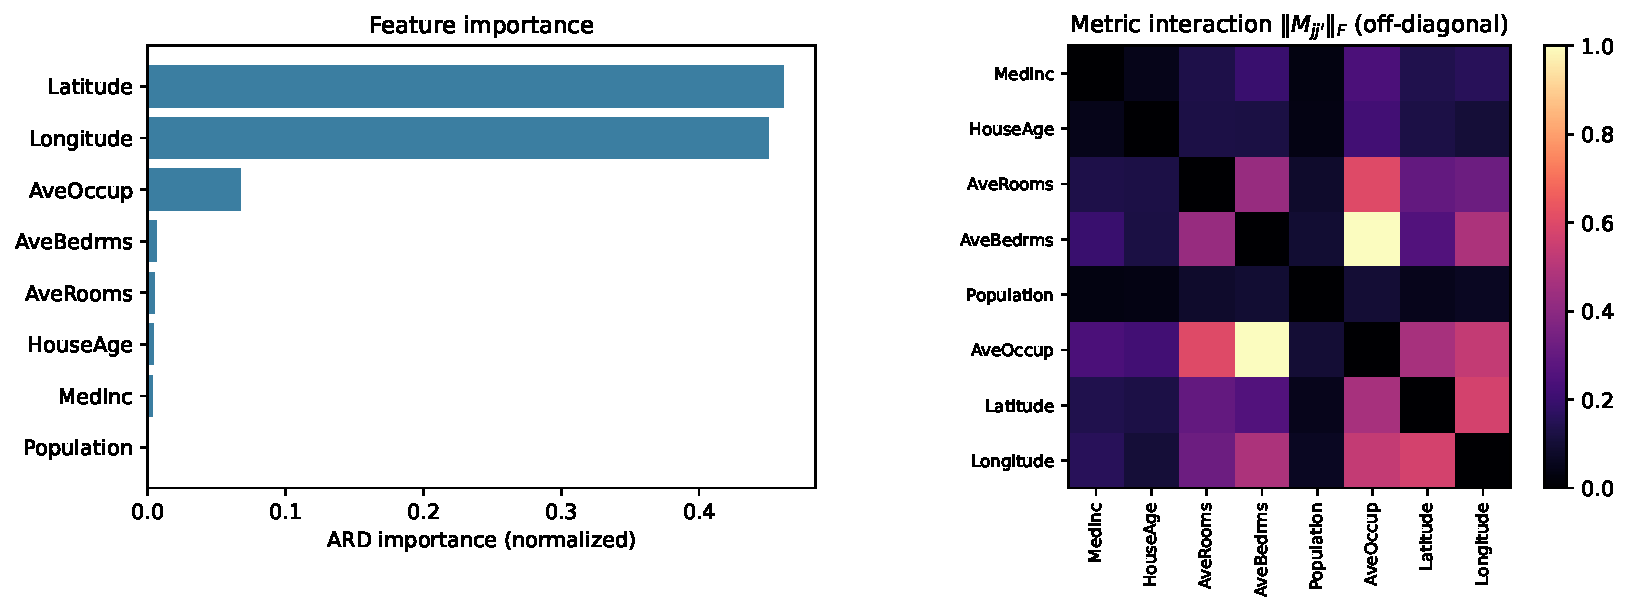
\includegraphics[width=\textwidth]{figures/interpret.pdf}
\caption{ARD interpretability on California Housing, read directly from the fitted kernel
($H{=}4$, $K{=}8$). Left: per-feature importance $I_j$ of \eqref{eq:ardimp}. Right: metric
interaction $\|M_{jj'}\|_F$ between feature pairs, diagonal removed.}
\label{fig:interpret}
\end{figure}

\section{Related work}
Spectral-mixture \citep{wilson2013}, sparse-spectrum \citep{lazarogredilla2010} and \`a-la-carte
\citep{yang2015} kernels learn $d$-dimensional frequencies that couple all coordinates;
\eqref{eq:psi} is deliberately the opposite, additive before any mixing, with interactions
introduced by an inspectable operator. Non-stationary spectral kernels \citep{remes2017} relax
stationarity. Deep kernel learning \citep{wilson2016} warps inputs by a deep network and can
collapse \citep{ober2021}; our warp is shallow and linear by design, which restricts and exposes
the collapses rather than precluding them. The per-coordinate Fourier embedding is the periodic
numerical embedding of tabular deep learning \citep{gorishniy2022,ye2024}, here given a spectral
reading. Convex kernel fusion has the exact decomposition and oracle guarantees of the sum RKHS
\citep{aronszajn1950,berlinet2004,stein1981}. Gradient-boosted trees remain the tabular default
\citep{chen2016xgboost,ke2017lightgbm,prokhorenkova2018catboost,grinsztajn2022}.

\section{Discussion}
The ladder turns one model into a sequence of controlled questions. Interactions come from the
kernel, not the mixer; the mixer only rotates them. Multiple banks beat more frequencies only
because the convex fuse keeps a bandwidth per scale; a linear mixer over banks is one wider bank.
The per-band frequency count is the overfitting axis and the bank count the multi-scale axis.
These are not asymptotic claims but statements read off real data by lifting one restriction at a
time. Three directions remain: a broader multi-seed benchmark against gradient boosting, fusion
weights chosen by an unbiased risk estimate to inherit the oracle guarantee and a low-rank input
projection before the per-coordinate map for genuinely multivariate frequencies.

\bibliographystyle{plainnat}
\bibliography{references}

\end{document}
